\chapter{Extension to 3D}
\section{Elasticity Equation}
We now consider the original model from \autoref{ssec:GeneralSeasModel} with a three-dimensional domain and a two-dimensional fault. The antiplane shear assumption does not hold anymore and the Cauchy stress tensor $\mathbf{\sigma}$ has nonzero entries everywhere. This implies that the elasticity equation in \autoref{eq:GeneralElastostaticProblem} cannot be simplified to the Poisson problem anymore. \\

\subsection{Stress components at the fault}
In the general friction law \ref{eq:GeneralFrictionLaw}, the normal stress $\sigma_x$ acts as a factor to the friction coefficient and the shear stress $\tau$ contains two components $\tau_{xy}$ $\tau_{xz}$ in the direction of the slip rate. In terms of the Cauchy stress tensor, let us denote these three components by the vector $\mathbf{\bar{\sigma}}$. To calculate the Jacobian matrices of the system and to set up the second order ODE formulation, the partial derivatives with respect to both slip components $S_y$ and $S_z$ are required. Similarly to \autoref{sssec:Jacobian_ODE}, the partial derivatives $\pdv{u_{rs}}{S_{ln}}$, $\pdv{\mathbf{\bar{\sigma}}_{kp}}{u_{rs}}$ and $\pdv{\mathbf{\bar{\sigma}}_{kp}}{S_{ln}}$ have to be calculated to express the change in stress $\dv{\mathbf{\bar{\sigma}}_{kp}}{S_{ln}}$. Since the stress and the displacement $u$ acts in three dimensions over the indices $k$ and $r$, but the slip only in two over the index $n$, the final Jacobian is not a square matrix. \\
The term $\pdv{u_{sr}}{S_{ln}}$ is obtained by solving the discontinuous Galerkin problem with unit vectors instead of $S_{ln}$ without further source terms or boundary conditions. The stress $\mathbf{\hat{\sigma}}_{kp}$ at the quadrature points on one side of the fault and its derivative are calculated by:
\begin{align}
	\mathbf{\hat{\sigma}}_{pq} &= \lambda_q D_{lsq} u_{ls} n_{pq} + \mu_q \left(D_{ljq} u_{lp} n_{jq} + D_{lpq} u_{lj} n_{jq} \right) \\ \Leftrightarrow
	\pdv{\mathbf{\hat{\sigma}}_{pq}}{u_{rs}} &= \lambda_q D_{lsq} \pdv{u_{ls}}{u_{rs}} n_{pq} + \mu_q \left(D_{ljq} \pdv{u_{lp}}{u_{rs}} n_{jq} + D_{lpq} \pdv{u_{lj}}{u_{rs}} n_{jq} \right) \\ \Leftrightarrow
	\pdv{\mathbf{\hat{\sigma}}_{pq}}{u_{rs}} &= \lambda_q D_{rsq}  n_{pq} + \mu_q \left(D_{rjq} \delta_{ps} n_{jq} + D_{rpq} n_{sq} \right) \label{eq:intermediateStep7.3}
\end{align}
From \autoref{eq:intermediateStep7.3}, the term $\pdv{\mathbf{\bar{\sigma}}_{kp}}{u_{rs}}$ is obtained with the same further linear transformations that are applied from $\mathbf{\hat{\sigma}}$ to $\mathbf{\bar{\sigma}}$. Finally, the term $\pdv{\mathbf{\bar{\sigma}}_{kp}}{S_{ln}}$ is calculated in a similar fashion to \autoref{eq:JacobianDtauDS_Poisson}, under consideration of the correct dimensions. All together, the Jacobian matrix for the stress components with respect to the slip can be represented by the following block matrix.
\begin{equation}
	\label{eq:stressComponentsJacobian3D}
	\pdv{\mathbf{\bar{\sigma}}}{U}\pdv{U}{S}+ \pdv{\mathbf{\bar{\sigma}}}{S} = \dv{\mathbf{\bar{\sigma}}}{S} = \begin{pmatrix}
		\pdv{\sigma_x}{S_y} & \pdv{\sigma_x}{S_z}\\ 
		\pdv{\tau_{xy}}{S_y}  & \pdv{\tau_{xy}}{S_z} \\ 
		\pdv{\tau_{xz}}{S_y}  & \pdv{\tau_{xz}}{S_z}		
	\end{pmatrix}
\end{equation}
None of these entries depend on the current state of the system, the matrix can thus be pre-computed, as usual, in the initialization phase.

\subsection{Derivatives of the friction law}
The definition of the friction law in \autoref{eq:GeneralFrictionLaw} uses the absolute value of the shear stress and of the slip rate. As the components at the fault are two-dimensional, the euclidean norms of these quantities have to be computed before the friction law can be evaluated. This however complicates the Jacobian matrices $\pdv{F}{S}$ and $\pdv{F}{V}$, because the partial derivatives in both dimensions are now needed. We get:
\begin{equation}
	F(S,V,\psi) = \sqrt{\tau_{xy}^2 + \tau_{xz}^2} - \sigma_xf\left(\sqrt{V_y^2 + V_z^2},\psi\right) - \eta\sqrt{V_y^2 + V_z^2} 
\end{equation}
\begin{align}
	\label{eq:Jacobian_dF_dS_Elasticity3D}
	&\begin{cases}
		\pdv{F}{S_y} = \frac{1}{\norm{\tau}}\left(\tau_{xy}\pdv{\tau_{xy}}{S_y} + \tau_{xz}\pdv{\tau_{xz}}{S_y}\right) - \pdv{\sigma_x}{S_y}f(\norm{V},\psi) \\ 
		\pdv{F}{S_z} = \frac{1}{\norm{\tau}}\left(\tau_{xy}\pdv{\tau_{xy}}{S_z} + \tau_{xz}\pdv{\tau_{xz}}{S_z}\right) - \pdv{\sigma_x}{S_z}f(\norm{V},\psi) 
	\end{cases}
\end{align}
Unlike in the 2D problem, this term depends on the current state of the system and cannot be entirely precomputed. Luckily, it is obtained through linear transformations from the constant stress derivatives and the update is achieved in $\mathcal{O}\left(n^2\right)$. The vector of the slip rate is defined to always point in the direction of the shear stress on the fault. This motivates the introduction of a unit vector $u$ which always points in the current stress direction and whose components are:

\begin{align}
	u_y &= \frac{V_y}{\norm{V}} = \frac{\tau_{xy}}{\norm{\tau}} \\
	u_z &= \frac{V_z}{\norm{V}} = \frac{\tau_{xz}}{\norm{\tau}}
\end{align}

The unit vector gives the flexibility to be defined in the code either via the slip rate or the shear stress, preserving a consistent notation in the subsequent formulas. Further, the matrices $\mathbf{u_{y/z}}$ contain these components for each fault node on their diagonal. 
 
\section{Involved changes in the four formulations}
\subsection{First order ODE}
In the first order ODE formulation, the solution vector $x = (S_y, S_z, \psi)^T$ now contains two entries for the slip in $y$ and $z$ directions. The state variable $\psi$ remains of course a scalar quantity. The order of operations is not changed, thus at each evaluation of the right hand side, the absolute slip rate $\norm{V}$ is solved iteratively in the friction law with the norm of the shear stress. The $y$- and $z$-components of the slip rate are calculated by 
\begin{equation}
	\label{eq:update_V_3D}
	\begin{pmatrix}
		V_y \\ V_z
	\end{pmatrix} = \frac{\norm{V}}{\norm{\tau}} \begin{pmatrix}
													\tau_{xy} \\ \tau_{xz}
												 \end{pmatrix}
\end{equation}
and can be used for the right-hand side of the time derivatives $\dot{S}_y$ and $\dot{S}_z$. \\
For implicit methods, the Jacobian matrix has to be considerably adapted to split the derivatives with respect to the two fault dimensions. The Jacobians $\pdv{V_i}{S_j}$, where $i$ and $j$ stand for the two spatial directions $y$ and $z$ are calculated by derivating both sides of \autoref{eq:update_V_3D}.
\begin{align}
	\pdv{V_i}{S_j} =& \frac{\norm{V}}{\norm{\tau}}\pdv{\tau_{xi}}{S_j} + \frac{\pdv{\norm{V}}{S_j}\norm{\tau}-\norm{V}\pdv{\norm{\tau}}{S_j}}{\norm{\tau}^2}\tau_{xi} \nonumber\\ 
	=& \frac{\norm{V}}{\norm{\tau}}\pdv{\tau_{xi}}{S_j} + \mathbf{u_i}\left[-\left(\pdv{F}{V}\right)^{-1}\pdv{F}{S_j} - \frac{\norm{V}}{\norm{\tau}}\pdv{\sigma_{x}}{S_j}f(\norm{V},\psi)\right] 
	\label{eq:partial_V_S_Elasticity_3D}
\end{align}
where the Jacobian $\pdv{F}{V}$ has been previously calculated in \autoref{eq:partial_df_dV} and $\pdv{F}{S_j}$ is described in \autoref{eq:Jacobian_dF_dS_Elasticity3D}. Further, the derivative of $V_i$ with respect to the state variable and the derivatives of the ageing law $G$ are easily calculated as:
\begin{align}
	\label{eq:partial_dV_dpsi_elasticity_3D}
	\pdv{V_i}{\psi} &= \mathbf{u_i}\pdv{\norm{V}}{\psi} & &\text{using \autoref{eq:partial_V_psi}} \\
	\pdv{G}{S_j}    &= -\frac{b}{L}\left(\mathbf{u_y}\pdv{V_y}{S_j} + \mathbf{u_z}\pdv{V_z}{S_j}\right) & &\text{using \autoref{eq:partial_V_S_Elasticity_3D}} \\
	\pdv{G}{\psi}    &= -\frac{V_0}{L}e^{\frac{f_0 - \psi}{b}} -\frac{b}{L}\pdv{\norm{V}}{\psi} & & \text{using \autoref{eq:partial_V_psi}}
\end{align}

\subsection{Extended DAE}
For the extended DAE formulation, the solution vector $x = (S_y, S_z, \psi, V)^T$ also splits the slip in $y$ and $z$ components. The friction law in the last entry of the left-hand side function solves for the absolute value of the slip rate on each fault node. The separation in two components, needed for the derivatives $\dot{S}_y$ and $\dot{S}_z$ of the slip, are obtained from the direction of the shear stress as described in \autoref{eq:update_V_3D}. The Jacobian matrix contains the terms, with the shift $\sigma$ from the numerical scheme:
\begin{equation}
	\begin{pmatrix}
		\pdv{V_y}{S_y}-\sigma\mathbf{I} & \pdv{V_y}{S_z}                  & \mathbf{0}                      & \pdv{V_y}{V} \\
		\pdv{V_z}{S_y}                  & \pdv{V_z}{S_z}-\sigma\mathbf{I} & \mathbf{0}                      & \pdv{V_z}{V} \\ 
		\mathbf{0}                      & \mathbf{0}                      & \pdv{G}{\psi} -\sigma\mathbf{I} & \pdv{G}{V}   \\
		\pdv{F}{S_y}                    & \pdv{F}{S_z}                    & \pdv{F}{\psi}                   & \pdv{F}{V}
 	\end{pmatrix}
\end{equation}
The derivatives in the last column are all with respect to the absolute slip rate, and for the first two terms,  the derivatives are equal to the respective direction components $\pdv{V_y}{V} = u_y$ and $\pdv{V_z}{V} = u_z$. Further, the first two entries of the last row are exactly the matrices described in \autoref{eq:Jacobian_dF_dS_Elasticity3D}. Another novelty are the derivative terms $\pdv{V_i}{S_j}$ in the upper left corner. They are calculated the same way as in \autoref{eq:partial_V_S_Elasticity_3D}, but without the the derivative term with respect to the absolute slip rate:
\begin{equation}
	\pdv{V_i}{S_j} = \frac{\norm{V}}{\norm{\tau}}\left(\pdv{\tau_{xi}}{S_j} - \mathbf{u_i}\pdv{\sigma_x}{S_j}f(\norm{V}, \psi)\right)
\end{equation}
All other terms are scalar valued and are identical to the Jacobian of the two-dimensional Poisson problem derived in \autoref{sssec:Jacobian_DAE}. \\
The trick described in \autoref{ssec:iterative_solver_Jacobian} to effectively apply the iterative linear system solver on the dense subsystem and obtain the remaining entries by backward substitution is only of limited interest here, because the matrix now has six dense entries on three lines. Only the third block line may be eliminated.

The compact DAE formulation was not implemented with the 3D elasticity equation because of the observed convergence failure during earthquakes in the 2D scenario and its very similar behaviour to the extended DAE everywhere else. Moreover, it cannot be defined as straightforward in 3D, because the slip now has two components, but only one of them can be replaced by the friction law. 

\subsection{Second order ODE}
Finally, the most important task of this chapter is to get the best of all formulations, the second order ODE working in 3D. As the slip rate in the solution vector now directly stands for the derivative of the slip, we need both directional components and thus we have $x = (S_y, S_z, \psi, V_y, V_z)^T$. The same approach as in \autoref{eq:partial_V_S_Elasticity_3D} is followed to set up the time derivative $H$ of the slip rate. We get, for $i=y/z$:
\begin{align}
	H_i(\psi,V) &= \dv{V_i}{t} = \frac{\norm{V}}{\norm{\tau}}\dv{\tau_i}{t} + u_i\left(\dv{\norm{V}}{t} - \frac{\norm{V}}{\norm{\tau}}\dv{\norm{\tau}}{t}\right) \\
	&\text{with:}\qquad\begin{cases}
		\dv{\norm{V}}{t} = -\left(\dv{F}{V}\right)^{-1}\left[\pdv{\norm{\tau}}{t} - \pdv{\sigma_x}{t}f + \pdv{F}{S_j}\dv{S_j}{t} + \pdv{F}{\psi}\dv{\psi}{t} \right] \\
		\dv{\norm{\tau}}{t} = \pdv{\norm{\tau}}{t} + \pdv{\norm{\tau}}{S_j}\dv{S_j}{t} \\
		\dv{\tau_i}{t} = \pdv{\tau_i}{t} + \pdv{\tau_i}{S_j}\dv{S_j}{t}
	\end{cases}
\end{align}

Because the traction depends linearly on time, their partial derivatives can be precomputed once. Further, the partial derivatives of the slip rate in \autoref{eq:theLastLine} have already been stated in \autoref{eq:partial_V_S_Elasticity_3D} and \autoref{eq:partial_dV_dpsi_elasticity_3D}. As the value of the traction is not readily available but is needed in the ratio $\norm{V}/\norm{\tau}$, an alternative way to calculate this term is required. We know that, by definition, $\norm{\tau} = \sigma_x f + \eta\norm{V}$, and because the normal stress depends linearly of slip and time, we have $\sigma_x = \sigma_0 + \pdv{\sigma_x}{S_i}S_i + \pdv{\sigma_x}{t}t$. With this knowledge, first $\sigma$ and then $\norm{\tau}$ can be easily evaluated. Alternatively, it would have been possible to directly evaluate the shear stress components with the same method and calculate their norm $\norm{\tau}$. 

\section{Preliminary Results}
\subsection{Evolution of quantities}

To test the 3D implementations, a simulation with 30 fault elements has been performed over a duration of 250 years. \autoref{fig:timeEvolutionTANDEM_V_3D} shows the evolution of the maximum Euclidian norm of the slip rate for all available formulations in 3D. The same observations as for the 2D case in \autoref{sec:Results_EvolutionSlipRate} can be made: on a large time scale, all formulations behave the same, but when looking at the earthquake phase, the peaks from the different formulations occur with a certain delay. This time difference, up to 42 hours, is much larger than in 2D, where it \hfill remained \hfill below \hfill 40 \hfill seconds, \hfill and \hfill the \hfill implicit \hfill solutions \hfill for \hfill the \hfill 1st \hfill order 

\begin{figure}[H]
	\centering
	\begin{subfigure}[b]{0.32\textwidth}
		\centering 
		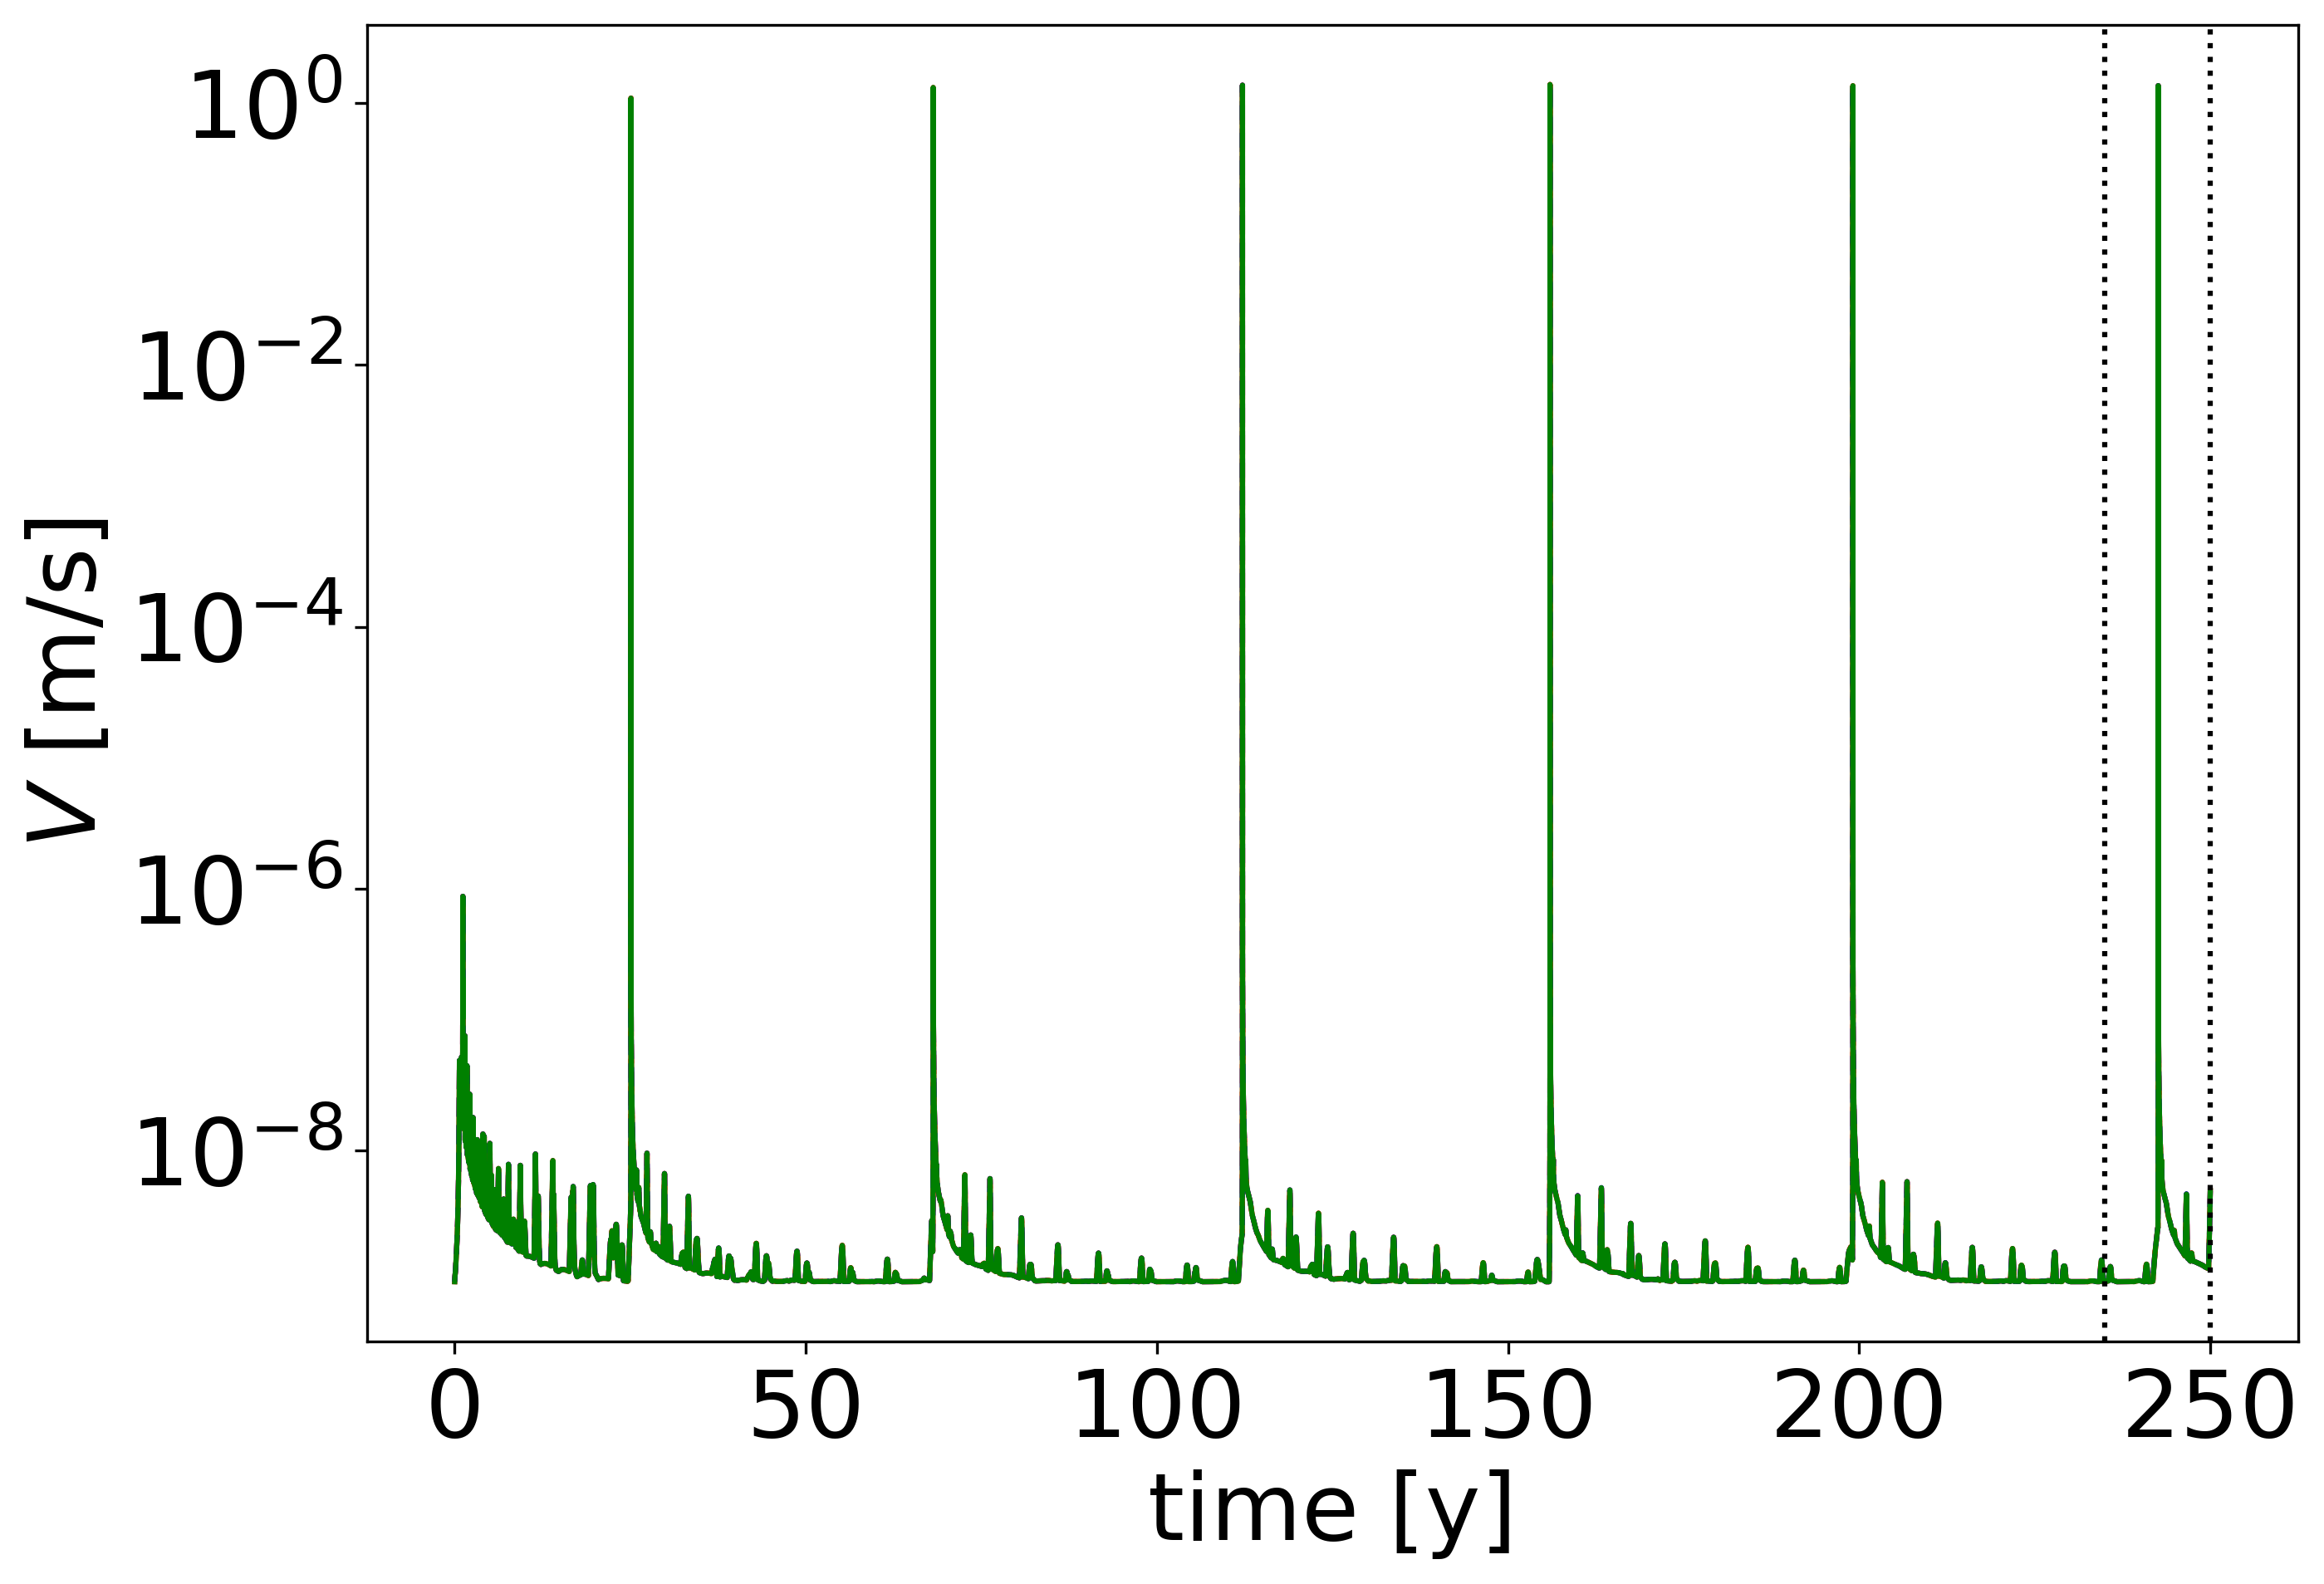
\includegraphics[width=1\textwidth]{images/TANDEMtimeEvolution_3D_maxSlipRate_allFormulations.png}
		\subcaption{Full simulation time \\ \ \\ \ } 
	\end{subfigure} 
	\begin{subfigure}[b]{0.32\textwidth}
		\centering
		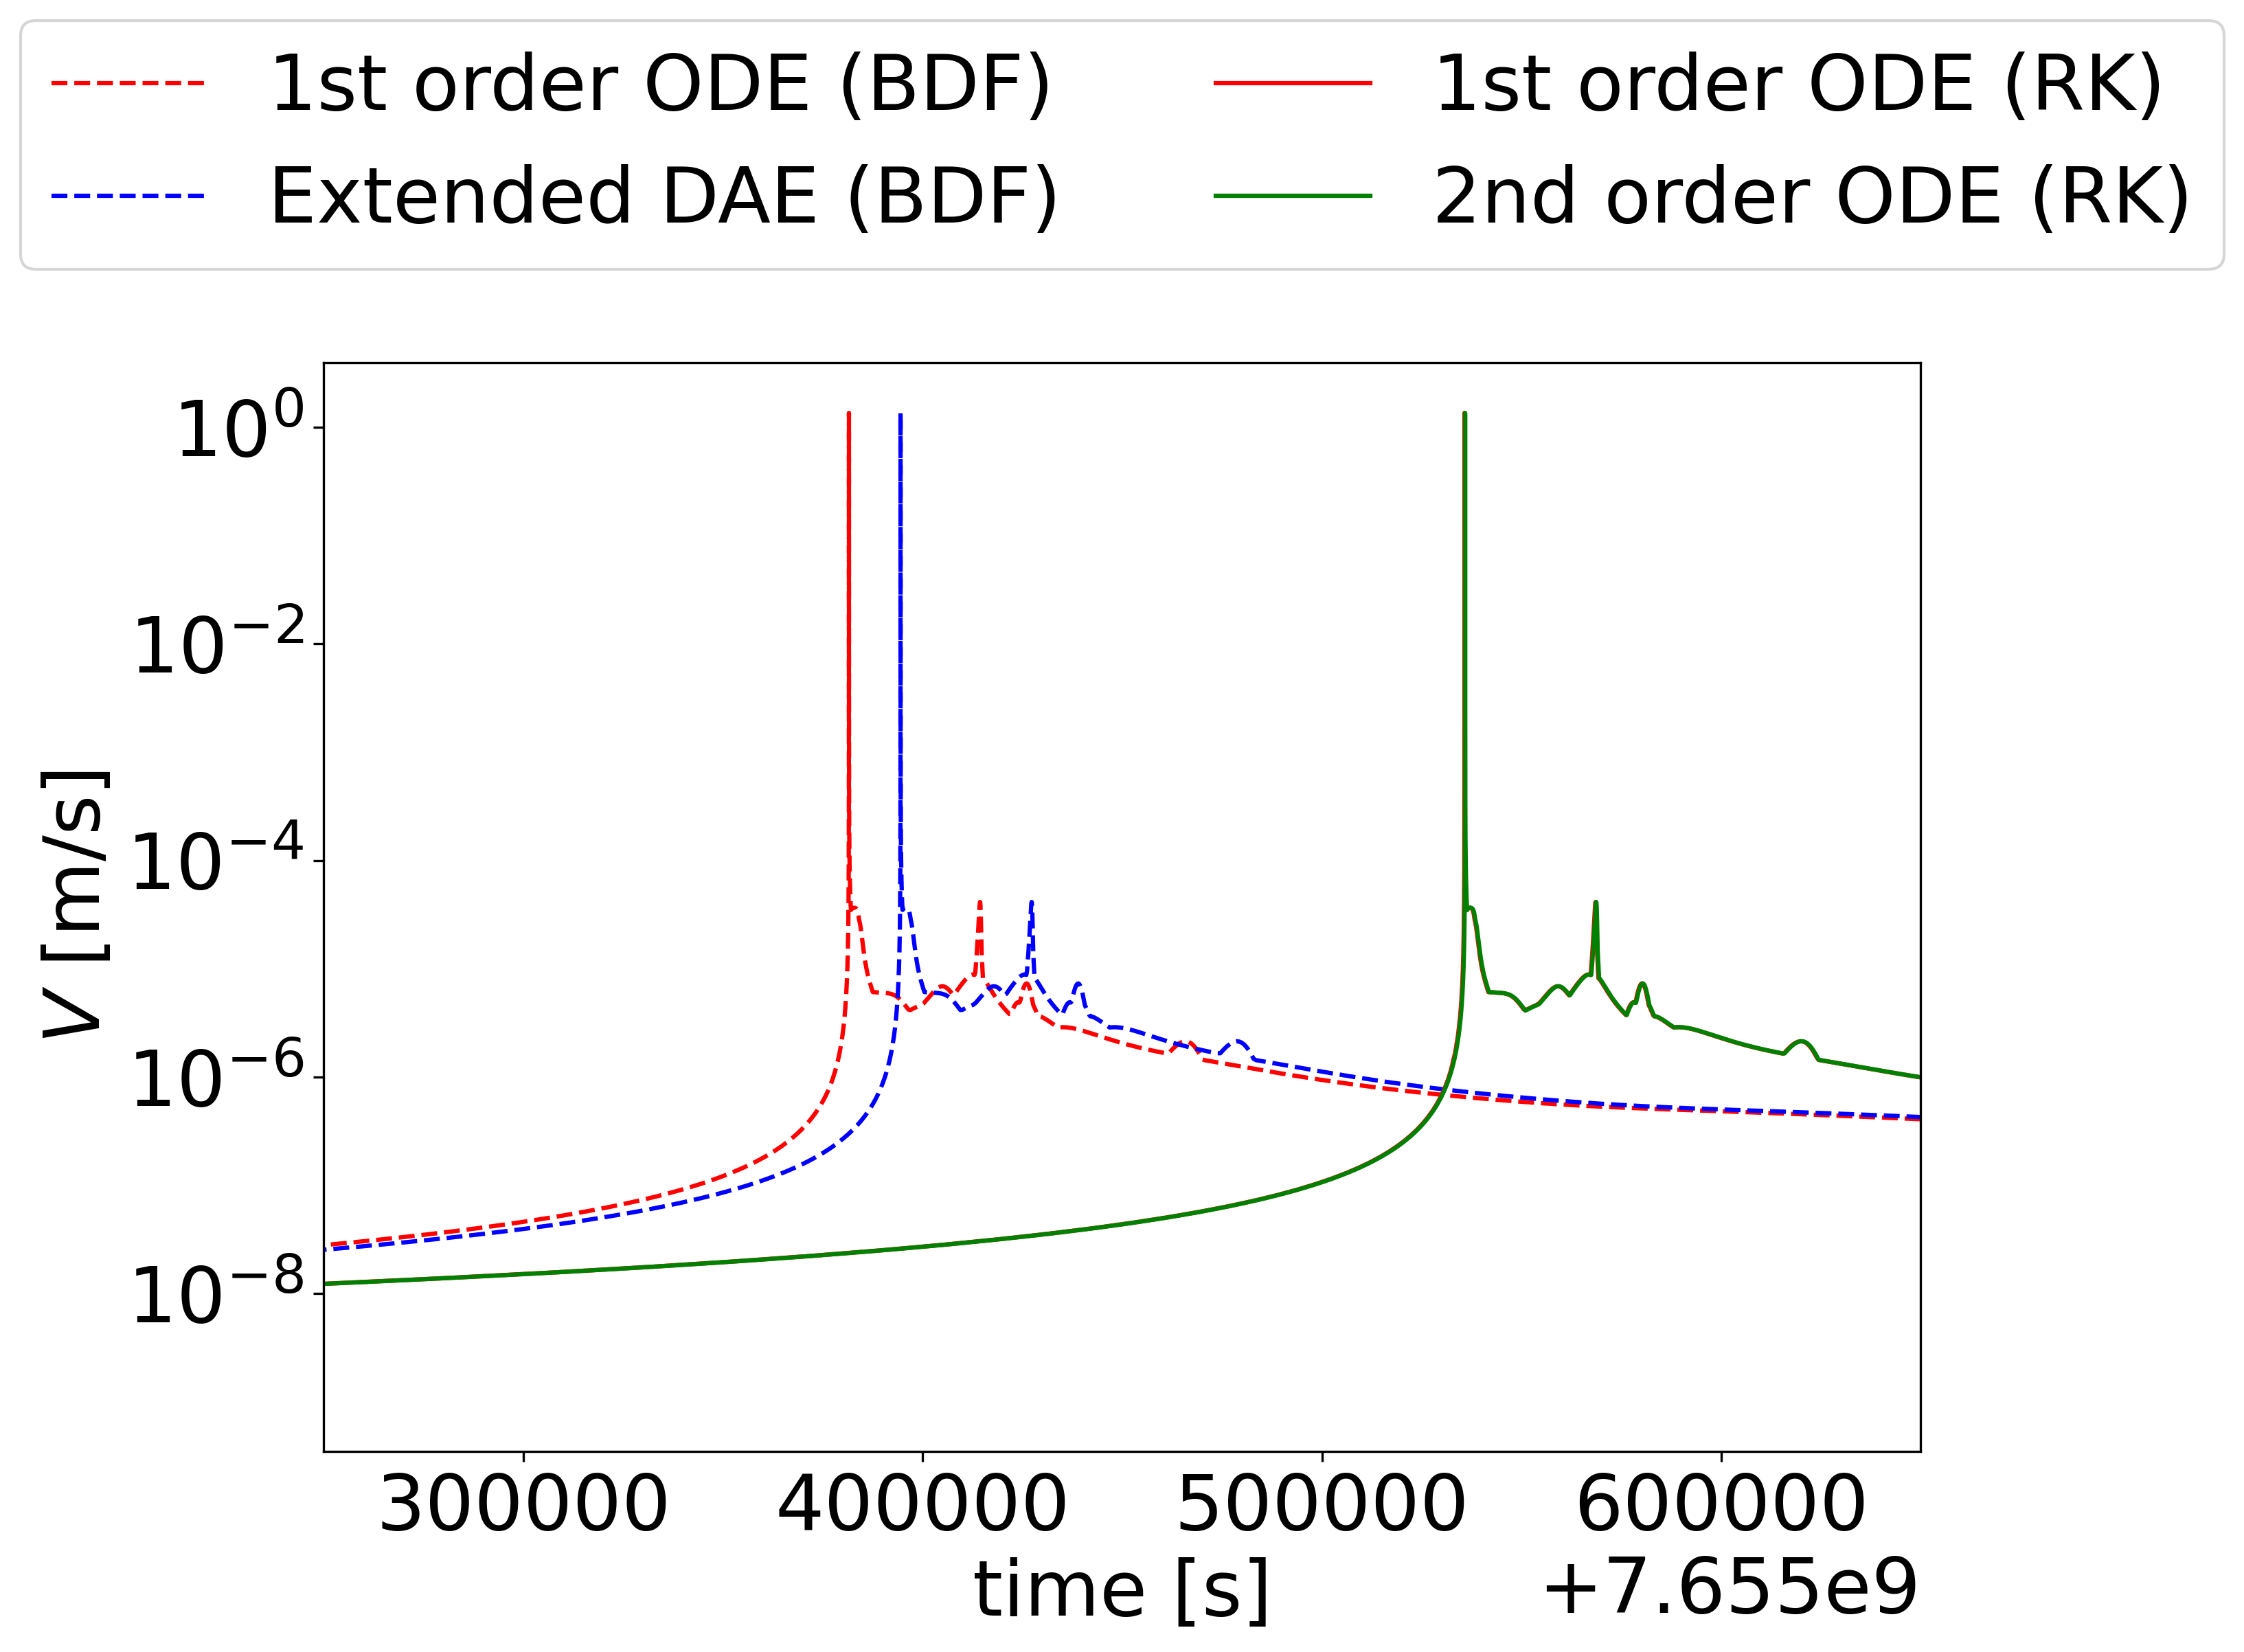
\includegraphics[width=1.18\textwidth]{images/TANDEMtimeEvolution_3D_maxSlipRate_allFormulations_LastEarthquake.png}
		\subcaption{Zoom onto the last earthquake \\ \ } 
	\end{subfigure}
	\begin{subfigure}[b]{0.32\textwidth}
		\centering
		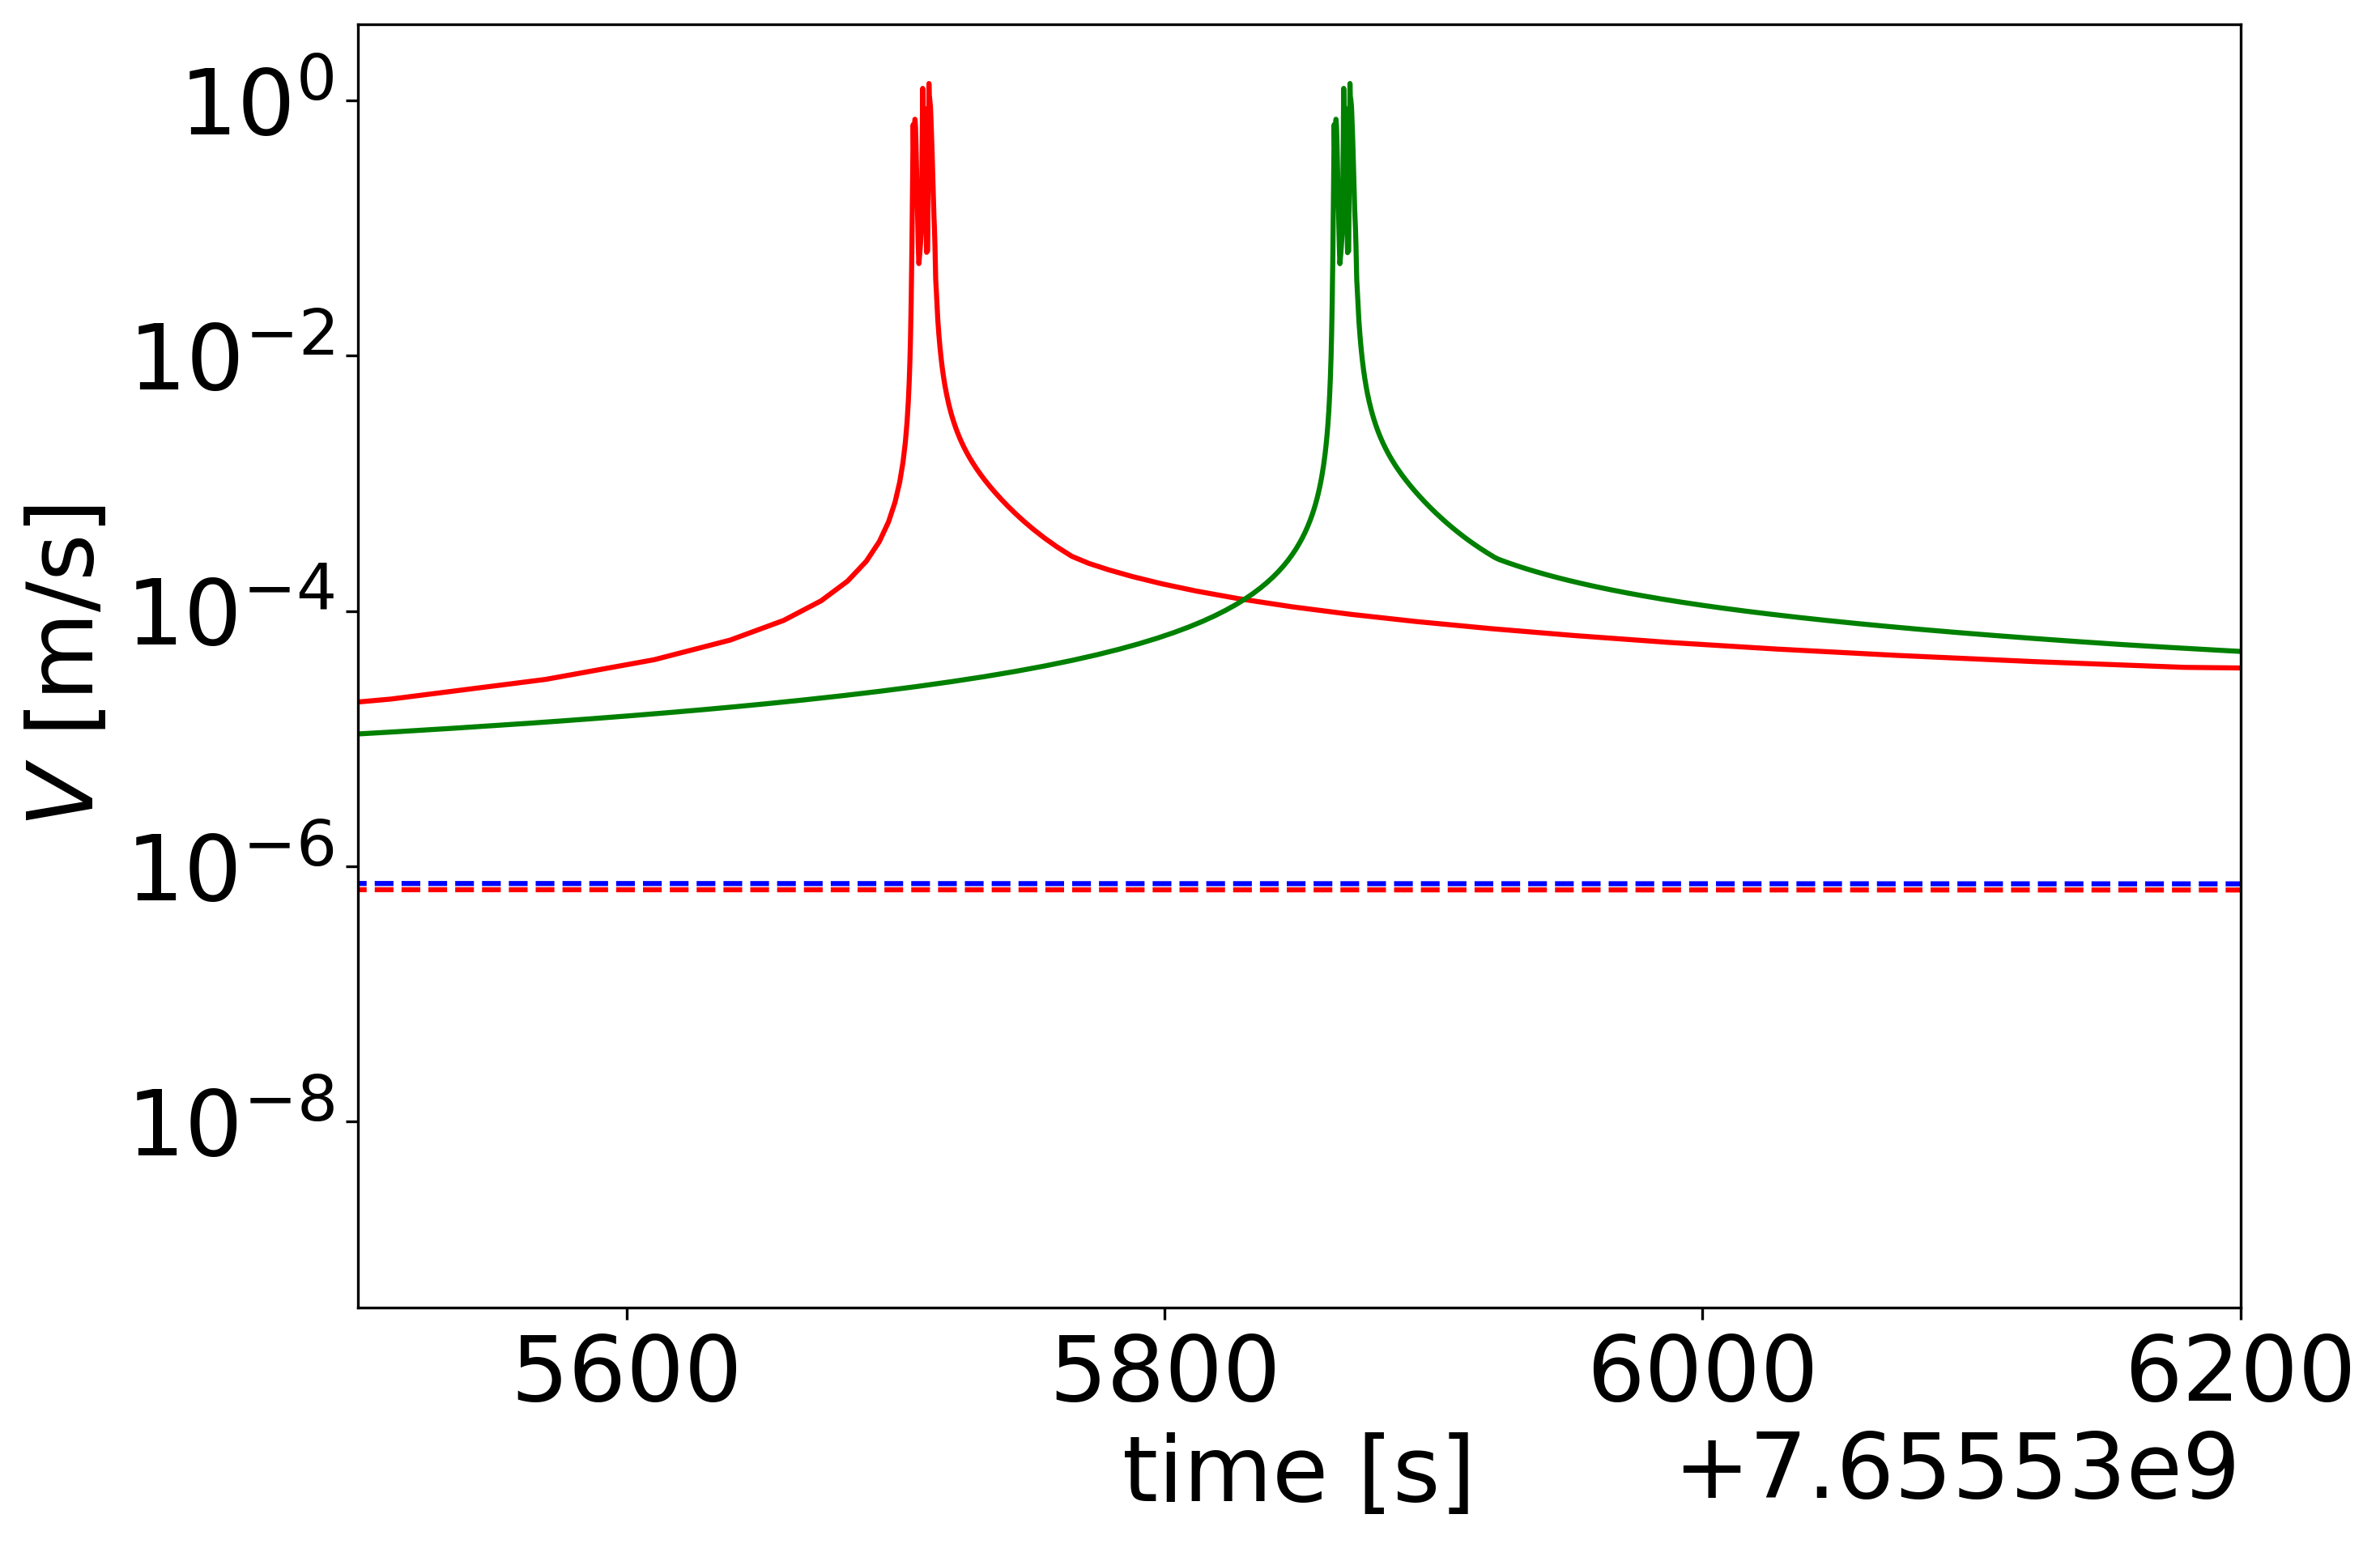
\includegraphics[width=1\textwidth]{images/TANDEMtimeEvolution_3D_maxSlipRate_allFormulations_LastEarthquake_Explicit.png}
		\subcaption{Zoom onto the explicit methods in the last earthquake}
	\end{subfigure}
	\caption{Evolution of the maximal slip rate $V$ on the fault for different solvers on the symmetric two-dimensional BP1 problem with 30 elements on the fault}
	\label{fig:timeEvolutionTANDEM_V_3D}
\end{figure}

\noindent formulations do not match perfectly anymore. Over the total simulation time of 250 years, much more earthquakes occur than in 2D and between the major peaks, many smaller ones indicate falsely detected earthquakes. All these observations do not mean that the 3D scenario is necessary less accurate, as these bad results most likely from the small number of fault elements: 30 fault elements discretize the entire two-dimensional interface between tectonic plates, whereas in 2D, 200 fault elements where used for a one-dimensional interface. However, a better fault resolution in 3D is not affordable in the current serial implementation of SEAS, this is why an efficient parallelization is crucial for meaningful three-dimensional simulations.

\subsection{Performance metrics}
For the simulations from the previous section, some performance results are given in \autoref{tab:performance_3D}. 

\begin{table}[H]
	\centering 
	\begin{tabular}{ | c | c c c c |}
		\hline	
		& 1st order ODE 	& 1st order ODE 	& extended DAE  & 2nd order ODE  	\\ 
		& (RK)				& (BDF) 			&  (BDF) 		& (RK) 		  	 	\\ \hline
		CPU time in solving
		& 62 978s 			& 34 099s			& 33 118s 		& 2 587s			  	\\  
		Number of timesteps 	
		& 41 361 		 	& 34 118			& 34 289		& 74 561				\\\hline
	\end{tabular}
	\caption{Some performance results for the 3D simulation}
	\label{tab:performance_3D}
\end{table}

As expected, the 2nd order ODE does not solve the DG problem, and has therefore a much lower CPU time in the solving phase than the other formulations. However, it requires about twice as many timesteps to finish the simulation. Among the first order formulations, the two implicit methods perform again very similarly, the extended DAE being slightly faster. The explicit RK method for the 1st order ODE formulation performs much worse than its implicit counterpart, which is due to the larger number of RHS evaluations per timestep and a larger total number of timesteps. Since the simulation has only been performed for one single fault resolution, no conclusions about the scalability can be drawn, but the observations match overall the findings in the 2D set-up from \autoref{sec:Results_Scalability}, so it can be expected that both domain dimensions scale the same way. 






